\section{Теоретические вопросы}
\subsection{Характеристика инвестиционного климата в России. Факторы, определяющие инвестиционный климат}

Высокая инвестиционная активность --- одно из условий развития экономики страны.
Она достигается за счет роста объемов реализуемых инвестиционных ресурсов и их целесообразного использования в различных сферах.
Инвестиции на новой научно-технической базе формируют производственный потенциал конкретной организации в целом, предопределяют конкурентные позиции России на мировых рынках.
Важную роль играет возможность привлечения иностранного капитала в виде прямых капиталовложений, портфельных инвестиций и других активов.
Это выполнимо только при условии хорошего инвестиционного климата в стране.

Инвестиционный климат --- совокупность  политических. экономических, юридических, социальных, бытовых и других факторов, которые предопределяют степень риска капиталовложений и возможность их эффективного использования.
инвестиционный климат зависит от инвестиционной активности и инвестиционной привлекательности (см. \ref{fig:invest})

\begin{figure}[h]
	\centering
	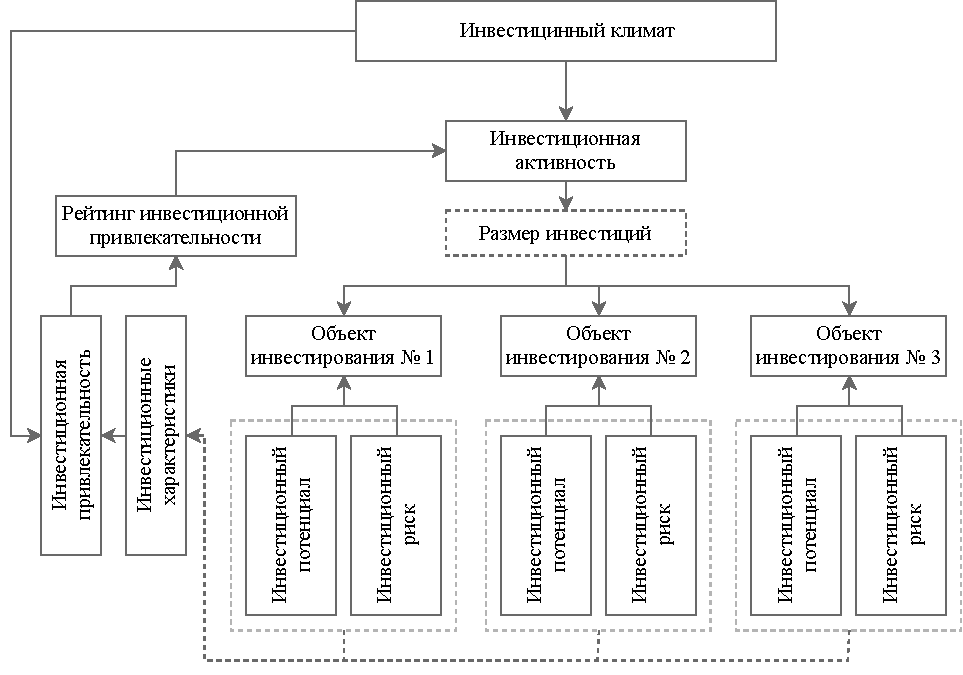
\includegraphics[width=1\linewidth]{invest}
	\caption{Взаимосвязь между инвестиционным климатом, инвестиционной активностью и инвстиционной привлекательностью}
	\label{fig:invest}
\end{figure}



















\subsection{Принципы оценки эффективности инвестиционного проекта}
\subsection{Основные мероприятия, направленные на снижение инвестиционных рисков в проектах}